% User guide: http://mirrors.ctan.org/macros/latex/contrib/bookcover/bookcover.pdf

\documentclass[
    coverwidth=21.6cm,
    coverheight=30.2cm,
    spinewidth=0.3cm,
    flapwidth=0cm,
    bleedwidth=5mm,
    marklength=5mm,
%    trimmed % Show only trimmed part!
    ]{bookcover}

%\bookcovertrimmedpart{front} % Trimmed part is the front cover
%\bookcovertrimmedpart{back} % Trimmed part is the back cover
%\bookcovertrimmedpart{spine} % Trimmed part is the spine

\newbookcovercomponenttype{center rotate}{
    \vfill
    \centering
    \rotatebox[origin=c]{-90}{#1}
    \vfill}

\usepackage{contour}
\usepackage{kantlipsum,microtype}
\usepackage{fontspec}
\usepackage{xcolor}

\definecolor{boi}{HTML}{d6bea0}

\begin{document}

\begin{bookcover}

%\begin{bookcoverelement}{picture}{bg whole}
%assets/boi_background.jpg
%\end{bookcoverelement}

\begin{bookcoverelement}{picture}{bg front}
assets/boi_cover.jpg
\end{bookcoverelement}

\begin{bookcoverelement}{center rotate}{bg back and spine and wrap}
 \makebox[\partwidth]{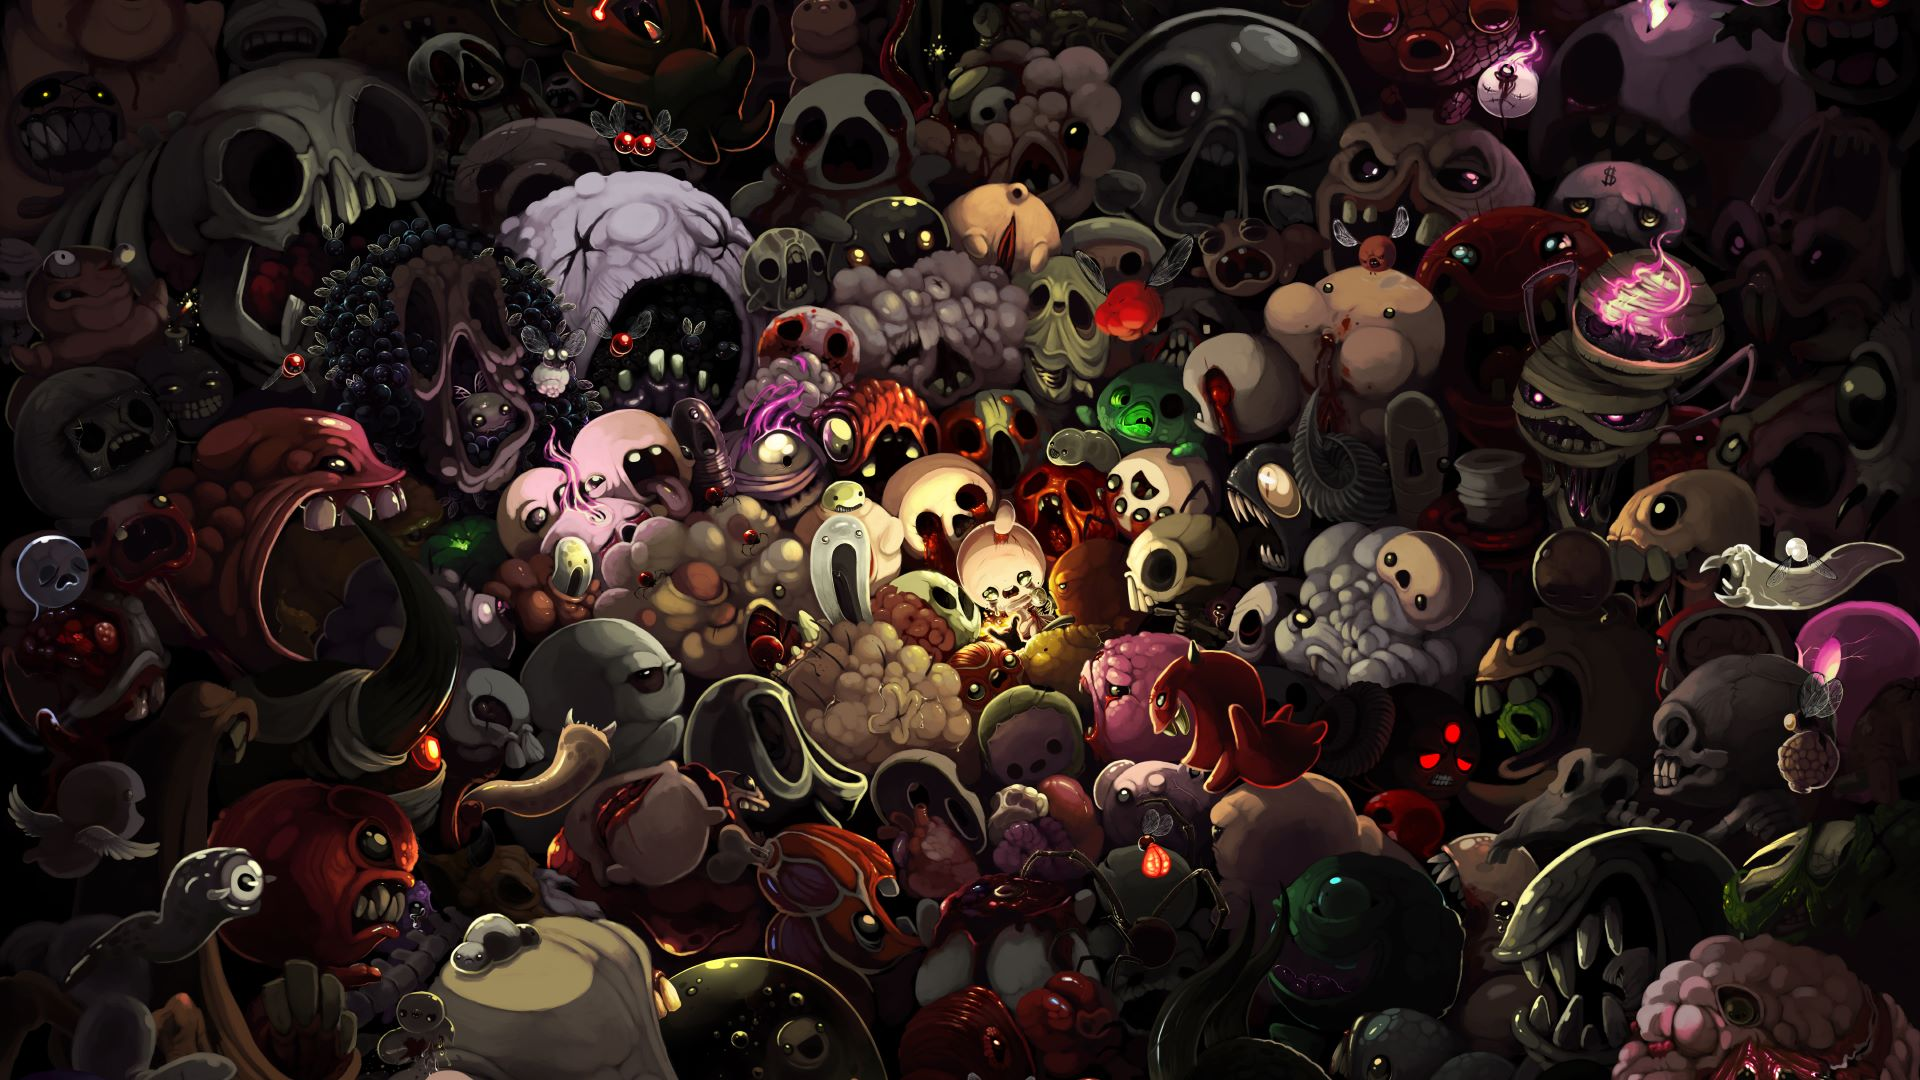
\includegraphics[height=\partwidth,keepaspectratio,clip]{assets/boi_background.jpg}}
\end{bookcoverelement}


% Picture on the front cover behind the title
%\begin{bookcoverelement}{picture}{front}[,0.5\partheight,,0.1\partheight]
%    assets/foursouls.png
%\end{bookcoverelement}

% Author and title on the front cover
\begin{bookcoverelement}{normal}{front}[,,,10.1cm]
    \centering
    \contourlength{1pt} %how thick each copy is
    \contournumber{20}  %number of copies    
    \contour{black}{\Huge\textbf{\textcolor{boi}{\fontspec{upheavtt.ttf} EXTENDED RULEBOOK}}}
\end{bookcoverelement}

%\begin{bookcoverelement}{normal}{front}[,,,11cm]
%    \centering
%    \contourlength{1pt} %how thick each copy is
%    \contournumber{20}  %number of copies
%    
%\end{bookcoverelement}

\end{bookcover}

\begin{bookcover}
\end{bookcover}

\end{document}